\documentclass[12pt]{article}
\usepackage[dvips]{epsfig}
\usepackage{color}
%e.g.  \textcolor{red,green,blue}{text}
\usepackage{url}
\usepackage[colorlinks=true]{hyperref}

\begin{document}

\section*{GENESIS: Documentation}

\section*{Introduction to Computational Neuroscience I}

\section*{Passive Membrane Properties}

\subsection*{Reverse engineering the brain}

Here, we introduce ways that computer simulation can be used as a tool for understanding the brain. Suggested background readings include \href{../bog-ch2/bog-ch2.pdf}{Chapters 2}, \href{../bog-ch3/bog-ch3.pdf}{3}, and \href{../bog-ch4/bog-ch4.pdf}{4} of {\it\,The Book of GENESIS: Exploring Realistic Neural Models with the GEneral NEural SImulation System} (commonly called the ``BoG''). 
%You can download or read the free internet edition at http://www.genesis-sim.org/GENESIS/iBoG/iBoGpdf. We won't have time to use the GENESIS simulator in this course during the short unit on realistic neural modeling, but I'll use slides and video clips of GENESIS simulations to illustrate some general ideas about this type of modeling.

The problem has been described as reverse engineering the brain (ref: Bower, 1995). As an analogy, suppose that we found an alien computer that was recovered from a crashed UFO. We'd like to understand how it works and learn what we can of its advanced technology.

There are various approaches we might take, for example, the high level systems approach--we can treat it as a black box and identify its input/output relationships. This corresponds to the psychological approach: the study of ``mind''. But, sooner or later, we have to understand the hardware.

We can try some circuit tracing and try to construct a wiring diagram. Unless it is a primitive single layer circuit board, this is hard--we may get incomplete knowledge. If we're lucky, we might be able to get some logic analyzer probes into critical pathways and try to figure out something from the relationships between the different pulse trains that we see.

Another problem--we may not be able to identify the components--no data book! There is just this rather insulting sticker that says ``no user serviceable parts inside''.

So, we will have to understand what the components do and how they work before we can understand their role in the circuit. As much as possible, we would like to understand the operation of simple subcircuits, such as the clock generator before we understand the whole system. This reductionist approach is basically the one we take in trying to understand the nervous system. We try to understand how the parts work and what they do, in order to understand the system as a whole.

In the case of the brain, we have several tools available, each with its limitations:

\begin{enumerate}

\item Imaging techniques (PET scans, MRI, etc.) or EEG--These have comparatively low resolution, but can help us create a ``block diagram''.

\item Neuron staining techniques--go back to Ramon y Cajal in the late 19th century--we can identify components and connections, to some extent, but we may have to make shrewd guesses and look for ways to test them.

\item Confocal microscopy gives us a 3-D view of individual neurons.

\item Radioactive tracers can map axonal connections.
 
\item Intra- and extracellular recording--simultaneous multicellular recording is analogous to using a logic analyzer.

\item Patch clamp techniques allow recording from individual ion channels.
 
\item Voltage sensitive dyes that change color according to the membrane potential, or dyes that are sensitive to the concentration of calcium ions.

\end{enumerate}

The technique that we introduce here is biologically realistic computer simulation. This approach falls under the heading of ``Computational Neuroscience''.
%I'll give some examples of this approach in the simulations that I'll show in these lectures.

Computational neuroscientists often disagree about the amount of biological realism that is required. Why make detailed biologically realistic models, rather than simpler abstract models that try to get right to the important behavior of the system of interest? The brain has trillions of neurons, with complicated branching dendrites, and dozens of different types of ion-selective channels. It's a natural reaction to fear that if we get too bogged down in the details, we'll spend years trying to understand calcium diffusion in dendrites, or the behavior of some esoteric type of channel, and never get to the goal of ``modeling the brain''.

It is tempting to make high-level abstract models without spiking neurons, hoping to discover some general principles of ``how the brain compute''. For example, some people use mathematical models that treat the cortex as a collection of coupled oscillators, or use greatly simplified neurons that sum up their inputs and produce a binary output based on some simple criterion.

The problem with these sorts of models is that with enough ingenuity and adjustable parameters, you can almost always contruct a model with any given desired behavior. If you construct an artifical neural network that performs well at recognizing human faces, does this tell you anything about how your brain recognizes faces? If the model is detailed and biologically realistic, then experiments on the actual living system can greatly narrow down the choices that are made in creating the model.

There is another trap that it is easy to fall into when deciding to use computer models. An obvious way to use modeling is to construct a model that incorporates some particular hypothesis and do ``computer experiment'' on the model in order to see if it behaves like experiments on the biological system. If it does, you might claim that this is evidence in favor of your hypothesis. The trouble with this is that it suffers from some of the same problems as abstract models: the simulation may be just giving the results that it was designed to give, and you don't know if a different model might have done just as well. With enough assumptions and tweaking of parameters, there are lots of models that could generate reasonable agreement with experiment.

A better approach is to try to ignore your preconceived ideas about the cause of a particular behavior and try to build the best model of the system you are studying that you can. This means incorporating the best phsysiological data that you can get to model the system in detail. This often means modeling neurons down to fine details of dendritic structure, and modeling each kind of ion channel that is known to exist in the cell. This fosters a close relationship with experiment, because you will soon discover experiments that you need to do in order to get data to use to characterize some channel or membrane parameter.

Once you have done this, you often find that you have to fill in the gaps in your knowledge with some hypotheses. You might postulate some connections between neurons which you feel might be necessary; or the existence of some interneuron in order to provide a needed inhibitory input. Or, you might assume the existence of some type of ionic channel which has been observed in other types of neurons and which seem necessary to explain the behavior of the one you want to model. Then you use your simulation as a sort of breadboard to test out your ideas. If the new feature gives better agreement with experiment, then you have the motivation to perform experiments to see if it really exists.

Of course, there will always be some parameters that you have to estimate. Then you compare the behavior of the model with some``function-neutral" experiments like voltage or current clamp on a cell, or perhaps an electric shock to a nerve in a system. You can then ``tune" the model by fitting any unknown parameters with data that isn't directly related to the behavior of interest. If the model passes these tests, then you can have more confidence in it. At this point you can start exploring the more interesting behavior of the model and understanding how the model produces this behavior. You can perform measurements and experiments on your model which might be impossible in the real system. Everything is accessible in a simulation. You can try to simplify your model in order to find out what features are important for the interesting behavior of the system--and which features are merely ``icing on the cake''.

You may discover that not only does the model behave like the biological system, but also that the mechanisms that you postulated are causing that behavior. But it is just as interesting to find that there is another cause, or even to see behavior in the model that you never thought to look for. This can be another useful way to guide the direction of experiments. This kind of realistic modeling opens up a new way to discover, through ``computer experiment'' the way that neurons process information.

\subsection*{Modeling a neuron}

So, how do we model a real neuron like this pyramidal cell or a network composed of them in the hippocampus?

\begin{figure}[h]
  \centering
 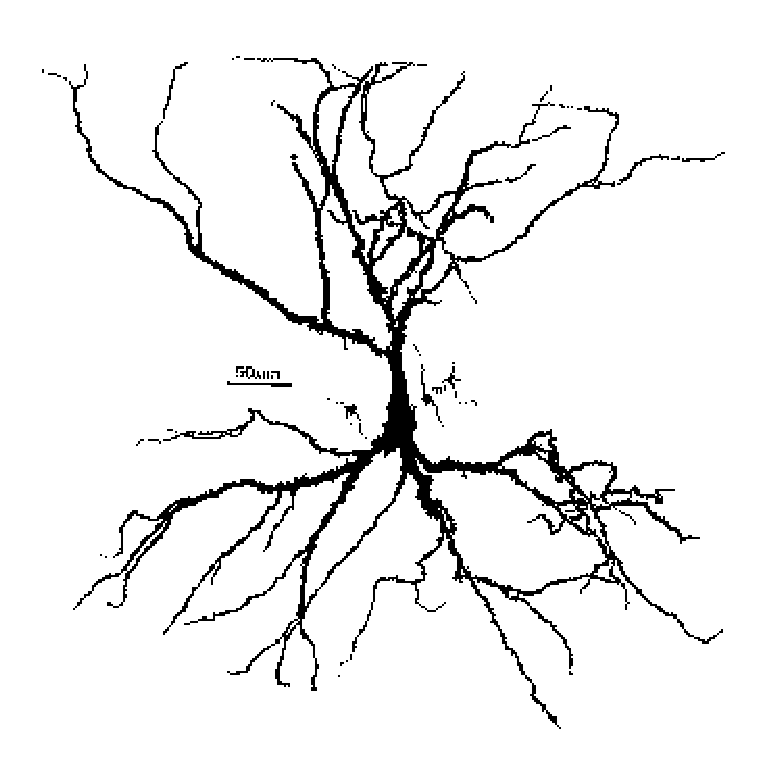
\includegraphics[scale=0.6]{figures/ca3smaller.eps}
%  \caption{}
  \label{fig:ca3smaller}
\end{figure}

As you can see, it doesn't look much like the ones you see in treatments of artificial neural networks, where you have a little circle with a summation sign inside. There are extensive trees of dendrites with the apical dendrites at the top, and basal dendrites at the bottom. Other neurons make synaptic connnections at various points on this structure, and release neurotransmitters that open channels, allowing ions to flow in or out of the cell, resulting in the production of post-synaptic potentials. It turns out that these dendrites play an important role in the processing of information by the cell. The pyramid shaped cell body, or soma, contains voltage activated sodium and potassium channels somewhat similar to those studied by Hodgkin and Huxley in the giant axon of the squid. Post-synaptic potentials produced in the dendrites can propagate to the soma to trigger action potentials. Throughout the cell, we also have passive channels that remain partly open all the time, leading to a leakage resistance. The insulating cell membrane separates the conductive cytoplasm inside the cell from the salt water environment outside, giving rise to a membrane capacitance. As the cytoplasm has some resistance, we also have an axial resistance along the dendrites and axon (not visible in this picture). Thus, a section of dendrite acts like a leaky cylindrical capacitor, coupled to neighboring sections with resistances.

In summary, we have a continuous distribution of resistance and capacitance across the membrane as well as an axial resistance parallel to the membrane. The various ion-selective channels across the membrane act like variable resistances.

The answer to our question is--we model it piece by piece. The usual approach is to model this with a lumped parameter model in which we divide the neuron into a finite number of compartments containing resistances, capacitances and batteries to represent ionic equilibrium potentials. We model this complex neuron with something like this.

\begin{figure}[h]
  \centering
 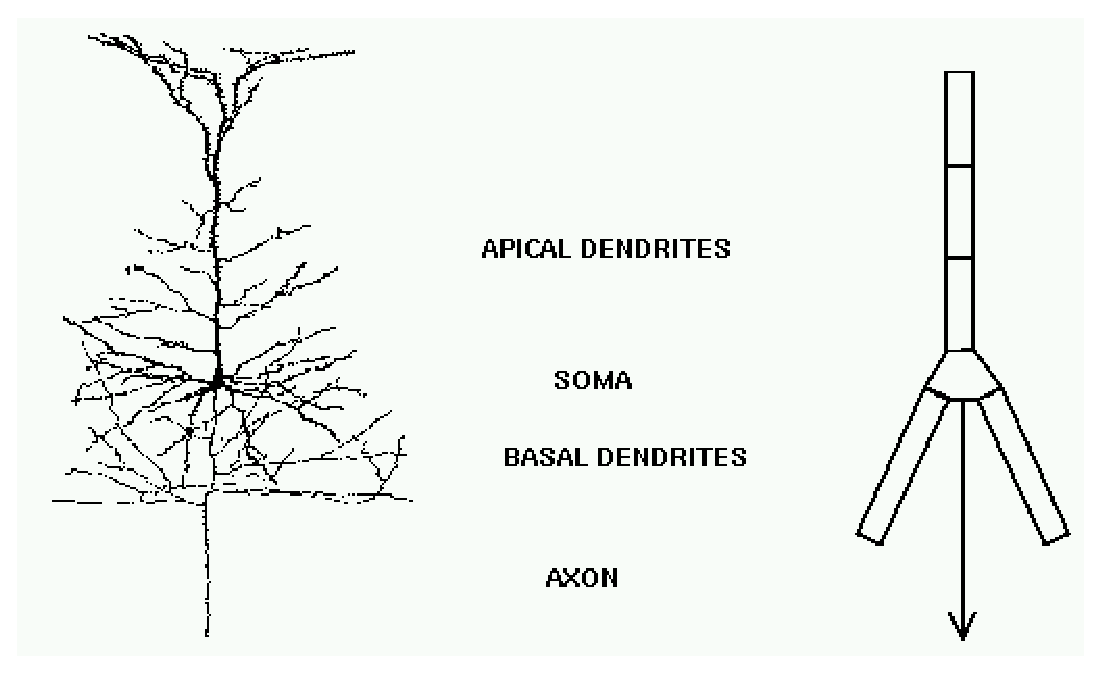
\includegraphics[scale=0.5]{figures/compartments.eps}
%  \caption{}
  \label{fig:compartments}
\end{figure}

Each of these compartments has an equivalent circuit, the properties of which we will explore further below.

\subsection*{Simplified vs. Detailed models}

As a contrast to this simple model with just a few compartments, here is a model of a Purkinje cell from the cerebellum, constructed with the GENESIS simulator by De Schutter and Bower (1994). It has 4550 compartments and 8021 active conductances (``channels"). If you look closely, you can see that it is actually composed of many cylinders.

\begin{figure}[h]
  \centering
 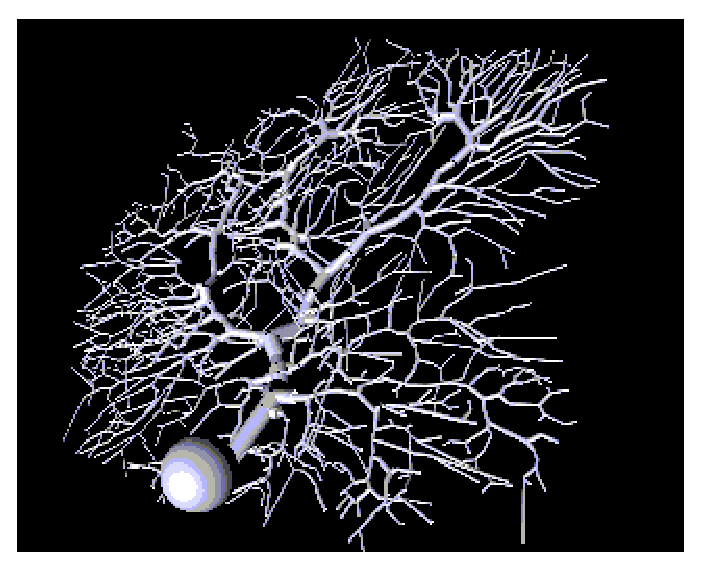
\includegraphics[scale=0.5]{figures/purkcell.eps}
%  \caption{}
  \label{fig:purkcell}
\end{figure}

Why would one need to construct such a detailed model? One reason is that, if the goal is to understand the way that individual neurons ``compute", rather than to implement some abstract model of ``neural computation", there is no way to avoid understanding the way that the dendritic structure processes its many inputs. After achieving this understanding with a structurally realistic model, it might be possible to produce a simpler ``ball and stick" model that will function equivalently in a large network model. If we ultimately want a simple, computationally efficient neuron model that can be used in simulations of very large neuronal networks, it is better to throw out details after proving that they aren't significant, rather than just hoping that we didn't omit something important at the outset. 

Sometimes this will lead to results that you wouldn't have expected. Here is an example from a computer simulation of the Purkinje cell, where false color is being used to represent the membrane potential throughout the cell. We can use this to find the effect of applying synaptic input at various places on the cell.

\begin{figure}[h]
  \centering
 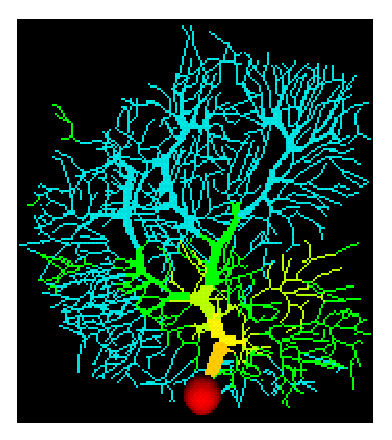
\includegraphics[scale=0.5]{figures/colpurk.eps}
%  \caption{}
  \label{fig:colpurk}
\end{figure}

It has been assumed for many years that dendrites process information ``locally", and that very local spatial and temporal patterns of activity sum, in some complicated way, to produce cell output. It was believed that inputs far from the soma would have comparitively little effect, because post-synaptic potentials would be greatly attenuated as they pass through the axial resistance of the dentritic tree to the soma. Modeling the cerebellar Purkinje cell suggests that the dendrite is actually operating globally--all regions of the dendrite have equal access to the soma, not as is usual, regions closer to the soma having a much larger influence. This comes about because a type of calcium channel found in the dendrites (p-type), amplifies granule cell inputs more at the distal dendrites than at proximal dendrites. This process would be very hard to understand, or even to predict, without a good computer model.

Here is a circuit diagram for a generic neural compartment.

\begin{figure}[h]
  \centering
 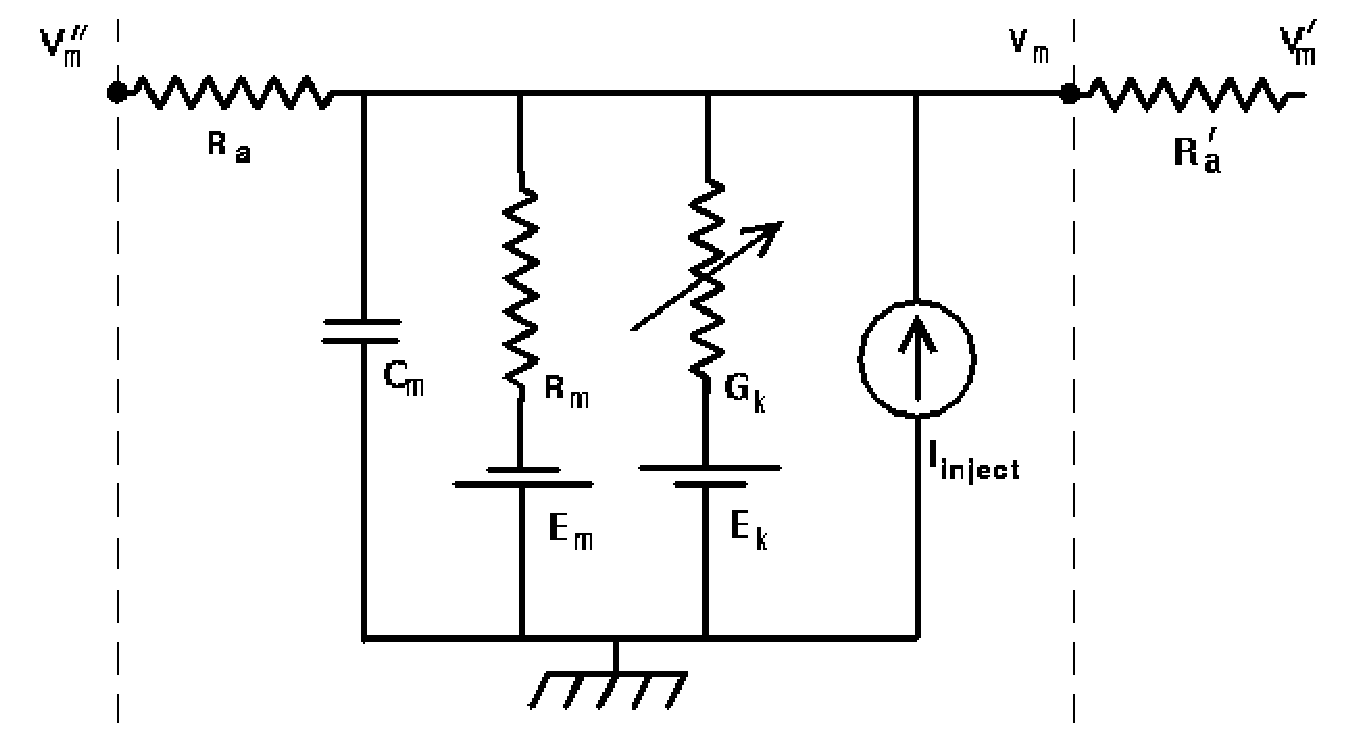
\includegraphics[scale=0.5]{figures/compt.eps}
%  \caption{}
  \label{fig:compt}
\end{figure}

$V_m$ represents the membrane potential at a point inside the compartment, relative to the ``ground" symbol outside the cell. The membrane capacitance $C_m$ can be charged or discharged as current flows into or out of the compartment, changing the value of $V_m$. This current can come from adjacent compartments, from the passage of ions through ion channels, or from a current $I_{inject}$ injected through a probe inserted into the compartment. Adjacent compartments have membrane potentials $V_m'$ and $V_m''$, and the difference in potential across the axial resistances $R_a$ and $R_a'$ can cause current to enter or leave the compartment. The ``leakage resistance" $R_m$ and its associated equilibrium potential $E_m$ represent the passive channels, and the resistor with the arrow through it represents one of the possible variable conductances that are specific to a particular ion or combination of ions. By convention, these are represented by a conductance $G_k$, rather than a resistance, $1/G_k$. Each one of these conductances has an associated equilibrium potential represented by the battery labeled $E_k$. The equilibrium potential (reversal potential) is the value of $V_m$ at which there is no net flow of the ion through the conductance. The values of the different $E_k$'s are calculated from the Nernst equation, where the Nernst potential of an ion of charge $z$, across a membrane, is determined by the concentration ratio in and outside the cell:

\begin{displaymath}
    E = \frac{R T}{z F} \ln\frac{[\mathrm{ions~outside~cell}]}{[\mathrm{ions~inside~cell}]}
\end{displaymath}

The greater this ratio, the greater the tendency for the ion to diffuse in one direction, and therefore the greater the Nernst potential required to prevent the diffusion. When the membrane is in thermodynamic equilibrium, i.e. there is no net flux of ions across the membrane, the membrane potential must be equal to the Nernst potential. However, in physiology, due to active ion pumps, the inside and outside of a cell are typically not in equilibrium. In this case the resting potential can be determined from the Goldman-Hodgkin-Katz or Goldman equation. For a membrane separating two $K_xNa_{1-x}Cl^-$ solutions, this is given by:

\begin{displaymath}
    E_{m, K_{x}Na_{1-x}Cl } = \frac{RT}{F} \ln{ \left( \frac{ P_{Na^{+}}[Na^{+}]_\mathrm{out} + P_{K^{+}}[K^{+}]_\mathrm{out} + P_{Cl^{-}}[Cl^{-}]_\mathrm{in} }{ P_{Na^{+}}[Na^{+}]_\mathrm{in} + P_{K^{+}}[K^{+}]_{\mathrm{in}} + P_{Cl^{-}}[Cl^{-}]_\mathrm{out} } \right) }
\end{displaymath}
where $E_m$ is the membrane potential, $P_{ion}$ the permeability for the given ion, $[ion]_{out}$ and $[ion]_{in}$ the extracellular and intracellular concentrations (respectively) of that ion, $R$ the ideal gas constant (8.314472\,J\,K$^{-1}$\,mol$^{-1}$), $T$ the absolute temperature in kelvins ($T =T_{^oC}$ + 273.15, e.g. at 25\,$^oC$, $T$ = 298.15\,$K$), and $F$ is Faraday's constant (the number of coulombs per mole of electrons: $F = 9.6485309\times10^4\,C$\,mol$^{-1}$). You can see that the Goldman equation is ``Nernst-like" but has a term for each permeant ion. The Nernst equation can be considered a special case of the Goldman equation for only one ion.

Typically, there will be several variable resistances, with different conductances and equilibrium potentials, corresponding to the different types of channels in the compartment. For example, the area near the region of the soma called the``axon hillock" may contain voltage dependent sodium and potassium channels, and regions in the dendrites are likely to contain channels that are chemically activated from synaptic connections. The index $k$ is being used here to represent one of these various types of conductances.

Electrical circuit theory tells us that the rate of change of the voltage across a capacitor is proportional to the net current that is applied to charge it. For the circuit above, the differential equation (DE) to be solved by the simulation software for each compartment is one that you may have seen before in elementary circuits courses:

\begin{displaymath}
		C \frac{dV}{dt} = I_{in} - I_{out}
\end{displaymath}

The full equation that this circuit obeys can be easily derived from Ohm's law and the circuit diagram:

\begin{equation}
		C_m \frac{dV_m}{dt} = \frac{(E_m-V_m)}{R_m}+\sum_k [G_k(E_k-V_m)]+\frac{(V_m'-V_m)}{R_a'} + \frac{(V_m''-V_M)}{R_a} +I_{inject}
\label{eq:eq1}		
\end{equation}

(You don't need to remember the equation, but take a minute to understand the origin of each of the terms, by comparing it to the circuit diagram.)

Of course, the $V_m''$ and $V_m'$ in the adjacent compartments affect the currents flowing into or out of the compartments, so we are solving many coupled DE's in parallel. Also, we will need good models for the way that the conductances vary with voltage, time or synaptic input. Usually, we can treat an axon as just a delay line for the propagation of action potentials, although it could also be modeled as a series of compartments if we were interested in understanding the details of axonal propagation of the action potential.

Hodgkin and Huxley used this approach to model a single compartment representing a short piece of squid giant axon. Since they did their work in the early '50s, they used hand crank mechanical calculators for the numerical integrations. We have a lot better tools now, and can solve harder problems, but the technique is essentially the same. If you have some programming experience, it would be fairly simple for you to to duplicate their model by writing a program in C, Java, or Matlab to solve the equations given in their papers. By using one of the freely available libraries for solving ordinary differential equations, you could even write your own neural simulator.

However, there are a lot of advantages to using a general purpose neural simulator and a high level simulation language, rather than writing your own simulation code in a computer programming language.

\begin{enumerate}
\item Built in tools - you don't have to write your own graphics display routines.

\item Designed to make it easy to add or subtract elements from your simulation--you don't have to go in and hack your code every time you want to make a change in your model.

\item A good simulator will also have a library of simulation components like neural compartments, ion channels, synapses, voltage clamp circuit components and other objects, which you can use in your simulations. 
\end{enumerate}

A lot of early neural modeling was done with SPICE--a general purpose simulator for electronic circuits. Now there are simulators that have been designed specifically for biologically realistic neural modeling.

These exmples were created with GENESIS, which was developed specifically for this type of modeling. If you want to find out more about GENESIS, or to download it and run some simulations, check the GENESIS web page, \href{http://www.genesis-sim.org/}{genesis-sim.org}. The other popular simulator for this type of modeling is called NEURON, available from \href{http://www.neuron.yale.edu/}{neuron.yale.edu}.

Here, we'll look at episodes from four different simulations. The first two are tutorial simulations designed to teach concepts in neuroscience, and the last two are GENESIS recreations of actual published research simulations.

\subsection*{The Hodgkin-Huxley Model}

Obviously, the place to start is with the Hodgkin-Huxley model. Their work, carried out in the early 1950's and described in a classic 1952 paper won them the Nobel Prize in 1963, and exemplifies a very good piece of modeling, combined with excellent experimental measurements. I can't emphasize this very necessary combination too strongly. Too many people get lost in a world of their own when doing computer modeling and lose touch with the world of experiment. Likewise, experimentalists may end up mindlessly gathering data without having a clear idea of how it will advance theoretical understanding.

Hodgkin and Huxley's model is at the basis of most single cell neuronal models. Most neurobiologists accept the importance of Hogkin and Huxley's work and their development of the voltage clamp technique without recognizing how important the modeling was to the work. Essentially, the model was what made them throw out their old way of looking at the changes in the membrane and introduce the new one. It is important to remember that at the time of their experiments, the modern concept of ion-selective channels controlling the flow of current through the membrane was only one of several competing hypotheses. Their model ruled out these alternative ideas, and also predicted the results of experiments that were not used in formulating the model.

Next, we will have a quick review of the Hodgkin-Huxley model, and then illustrate the model with some simulations.

The diagram below illustrates the ionic basis of the neuron membrane potential.

\begin{figure}[h]
  \centering
 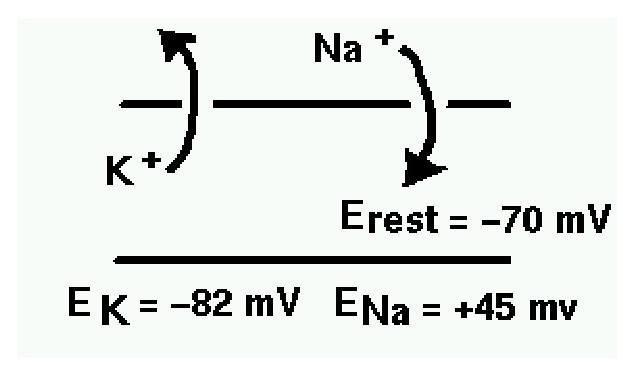
\includegraphics[scale=0.75]{figures/ionflow.eps}
%  \caption{}
  \label{fig:ionflow}
\end{figure}

It is known that the concentration of sodium ions is greater outside the cell, so they have a tendency to enter. The concentration of potassium ions is greater on the inside, so they tend to leave. Metabolic processes within the cell called ionic pumps maintain this balance of concentrations by ``pumping'' ions across the cell membrane. With this difference in ionic concentrations,  when the cell is at rest the interior of the cell is polarized to a membrane potential of about 70\,mV negative to the outside. Because of the higher exterior concentration of sodium, it has an equilibrium potential (reversal potential) of about 45\,mV positive with respect to the cell, meaning that it will tend to enter the cell as long as the membrane potential is less than $E_{Na}$. Likewise, this competition betweem osmotic and electrostatic forces means that potassium will tend to leave the cell unless the membrane potential falls below $E_K$. Note that these equilibrium potentials can be calculated from the Nernst equation, and the rest potential from the Goldman equation.

Hodgkin and Huxley quantitatively explained the process by which depolarization of the cell (an increase in $V_m$) causes $Na$-selective channels to open, allowing $Na$ ions to enter. This raises the potential, further increasing the conduction of the $Na$ channels, and causes the neuron to fire an action potential. Eventually, the $Na$ channels inactivate, and $K$-selective channels begin to open, causing a flow of charge out of the cell, ending or repolarizing the action potential.

Now, let's look at the mathematical model that describes this behavior. As before, we start with a circuit diagram. In this case, it is for a piece of squid giant axon.

\begin{figure}[h]
  \centering
 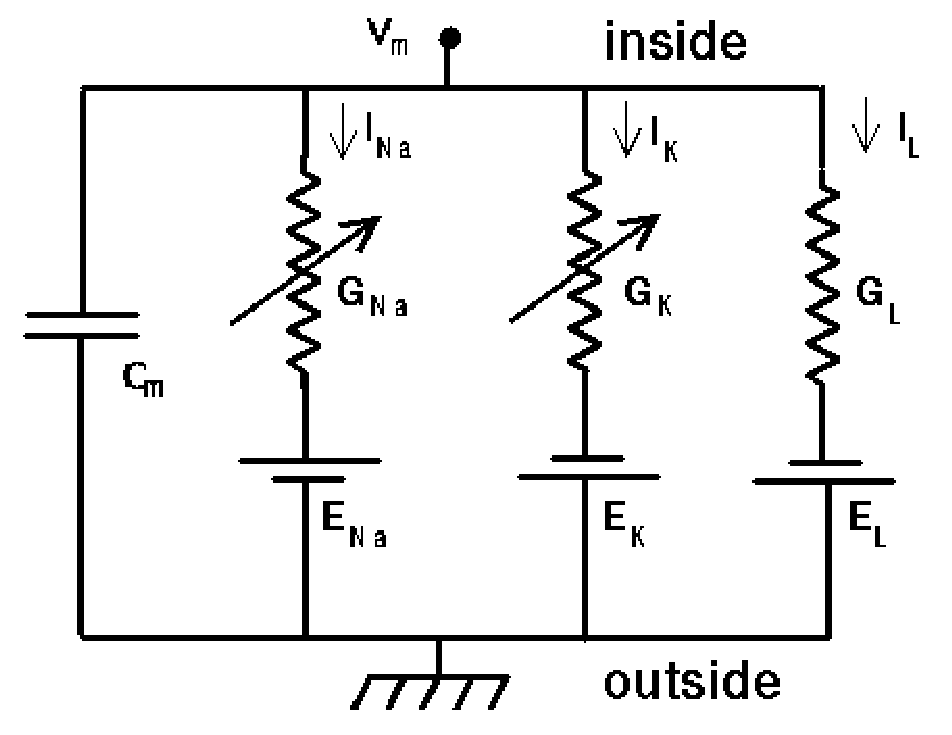
\includegraphics[scale=0.75]{figures/HHcompt.eps}
%  \caption{}
  \label{fig:hhcompt}
\end{figure}

Each of the two conductances $G_{Na}$ and $G_K$ represents the average effect of the binary gating of many ion channels.

The equation for $I_{in} - I_{out}$ is similar to the one for the``generic compartment" illustrated previously, but this is an isolated compartment, representing a piece of axon with the ends tied off in a Petri dish, so nothing is coming in through $R_a$. We have also shown the two different variable conductances representing the sodium ($G_{Na}$) and potassium ($G_K$) channels.

The hard part was to model the time and voltage dependence of the $Na$ and $K$ conductances. As you learned previously, the solution was to perform a series of voltage clamp experiments measuring both the total current and the current when the $Na$ conductance was disabled. They did this with an current injection probe, a current recording probe, and a feedback circuit or ``voltage clamp'' to insure that the injection probe applied just the right amount of current to hold the membrane potential at the desired value. They eliminated the sodium current by replacing the sea water with a solution containing choline instead of sodium chloride. Modern experiments use a puffer fish neurotoxin, tetrodotoxin (TTX) to block sodium channels.

By performing the experiments with different values of the clamp voltage, they were able to determine the time dependence and equilibrium value of the conductances at different membrane voltages. Here's a figure from one of their 1952 papers that shows the behavior of the $K$ conductance when the voltage is stepped to 25\,mV above the rest potential and then brought back down to the rest potential. For different clamping voltages, they found different values of the maxium conductance, and different time behaviors.

\begin{figure}[h]
  \centering
 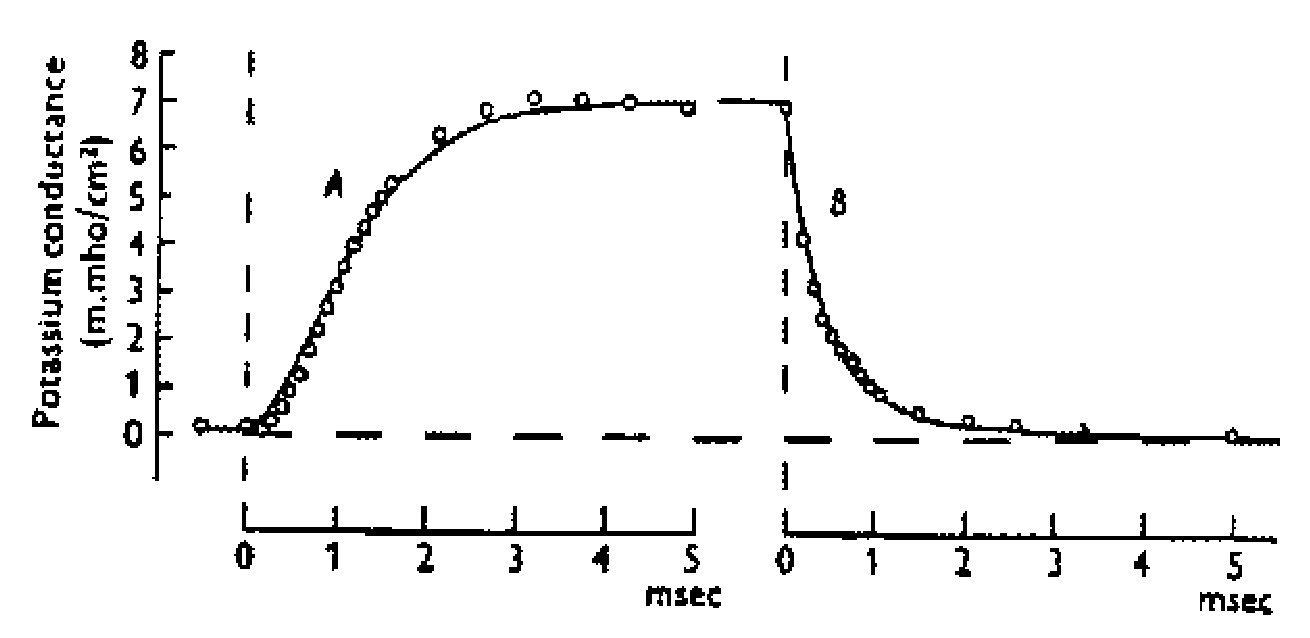
\includegraphics[scale=0.5]{figures/vcdata.eps}
%  \caption{}
  \label{fig:vcdata}
\end{figure}

It would be tempting to fit the rise and fall of the conductance to an exponential function of time, but the experimental measurements were best fitted by an exponential to the fourth power. They were able to fit the the $K$ conductance to an equation of the form

\begin{equation}
		G_K = \bar{g}_Kn^4
\label{eq:eq2}		
\end{equation}

Where $n$ is called the "activation variable" and has a simple exponential dependence governed by a single time constant, $\tau_n$:

\begin{equation}
		n(t) = n_\infty(V)-(n_\infty(V)-n_\infty(0))e^{-t/\tau_n}
\label{eq:eq3}		
\end{equation}

where $n_\infty$ is called the``steady state activation", i.e., the value reached by $n$ when the membrane is held at a potential $V$ for a long time. Hodgkin and Huxley were able to fit the voltage dependence of $n_\infty$ and $\tau_n$ to an analytic function of voltage involving exponentials.

The tricky part is that when we are dealing with action potentials rather than a voltage clamp, $n_\infty$ and $\tau_n$ are changing with the changing voltage, so we can't use this equation for $n$. Instead, we have to use a differential equation that has this solution when $V$ is constant,

\begin{equation}
		\frac{dn(V)}{dt} = \frac{(n_\infty(V) - n(V))}{\tau_n(V)}
\label{eq:eq4}	
\end{equation}

This makes things pretty hard if you are cranking out the numerical solution step by step on a calculator, but it's no big deal to solve on a computer. It is just one more simple DE to solve numerically.

Their fit for the $Na$ conductance was a little different, because they found that at a fixed voltage, the conductance rose with time and then decreased, so they had to fit it to a product

\begin{equation}
		G_{Na} = \bar{g}_{Na}m^{3}h
\label{eq:eq5}		
\end{equation}

Here, $m$ is the activation variable for $Na$, and $h$ is called the``inactivation variable" since it becomes smaller when $m$ becomes larger. The terminology is a little confusing though, because the conductance is large when the ``inactivation" is large. $m$ and $h$ obey equations just like the ones for $n$, but their steady state values and time constants have different voltage dependences. If you would like more information about the details of the model, see \href{../hh-model-details/hh-model-details.tex}{Further Details of the Hodgkin-Huxley Model}. The second part of this introduction to computational neuroscience can be found in  \href{../compneurosci-2/compneurosci-2.tex}{Introduction to Computational Neuroscience II}.

\subsection*{References:}

\begin{quote}

Bower, JM (1995) Reverse engineering the nervous system: An {\it in vivo}, {\it in vitro}, and {\it in computo} approach to understanding the mammalian olfactory system, {\it in} SF Zornetzer, JL Davis, and C Lau (eds.), {\it An Introduction to Neural and Electronic Networks}, 2nd edn., Academic Press, New York, NY, pp. 3--28.

\end{quote}

\end{document}
